\chapter{Wyznaczanie odpowiedzi skokowych}
Odpowiedz skokowa w algorytmie DMC oznacza odpowiedz obiektu na jednostkowy skok sterowania. Wyznacza się ją poprzez albo pobudzenie obiektu takim właśnie skokiem jednostkowym, albo, gdy jest to niemożliwe, jakimkolwiek innym i normalizowanie jej. W naszym przypadku nic nie stoi na przeszkodzie aby odrazu pobudzić obiekt takimi właśnie sygnałami.

\begin{figure}[h!]
	\centering
	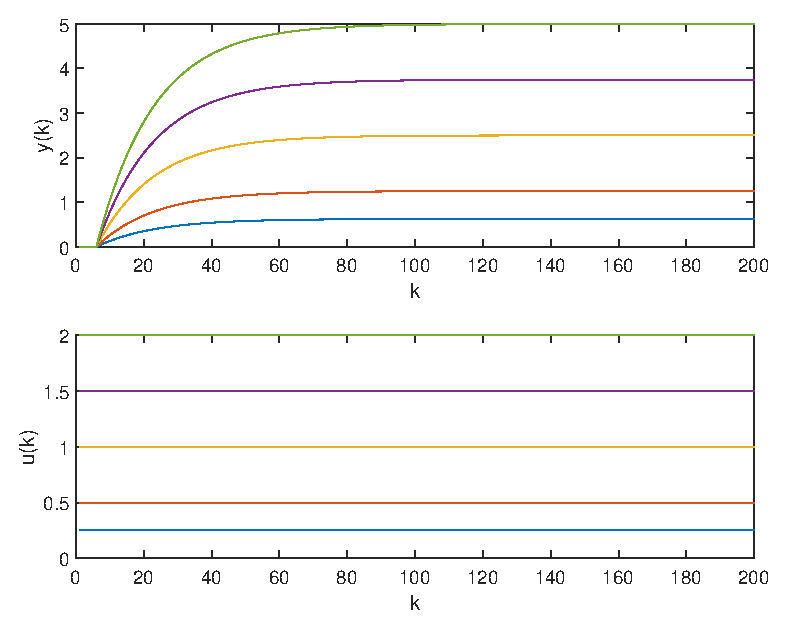
\includegraphics[scale=1]{Rys/odp_skok_u.eps}
	\caption{Odpowiedz skokowa obiektu pobodzonego jednotkowym skokiem sterowania$u$}
	\label{Rys:odp_skok_u}
\end{figure}
\begin{figure}[h!]
	\centering
	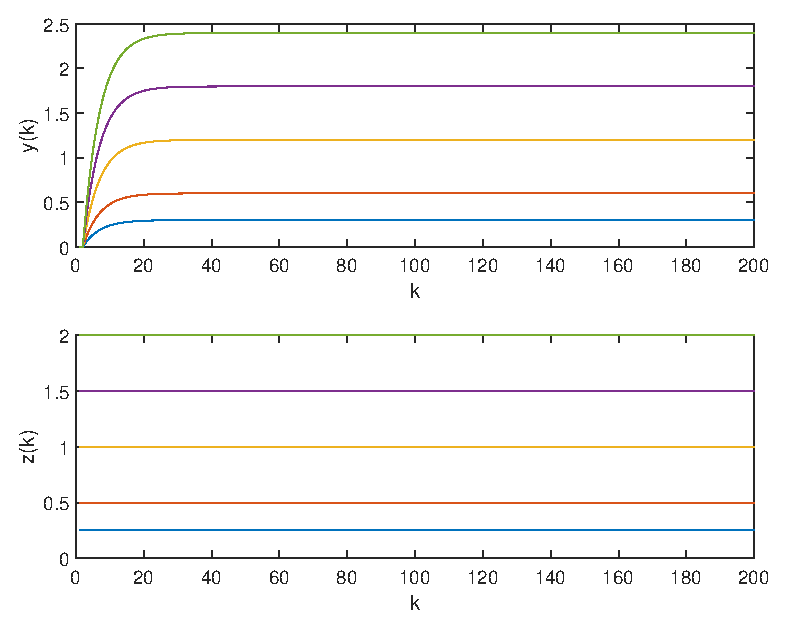
\includegraphics[scale=1]{Rys/odp_skok_z.eps}
	\caption{Odpowiedz skokowa obiektu pobodzonego jednotkowym skokiem sterowania$z$}
	\label{Rys:odp_skok_z}
\end{figure}